\section{Analyse der Bandlückenenergiebestimmung}
\subsection{Verfahren}
Das allgemeine Verfahren zur Bestimmung der Bandlückenenergie ist wie folgt:
Zum Beginn wurden zuerst die Messreihen vom Untergrund bereinigt und auf die Lampenenergie normiert. Hierzu wurde die Formel \ref{cleaner} verwendet. 
\begin{equation}
\label{cleaner}
\text{Trans}_{\text{Real}} = \frac{\text{\text{Trans }- \text{Untergrund}}}{\text{Lampe}_{\text{Trans}}} \qquad 
\text{Absorp}_{\text{Real}} = \frac{\text{\text{Absorp}- \text{Untergrund}}}{\text{Lampe}_{\text{Absorp}}}
\end{equation}
Nach dieser Korrektur wurden an den Stellen, wo Absorption und Transmission Gleichwahrscheinlich sind, Geraden angelegt und diese mit der Horizontalen des jeweiligen Maximum oder Minimum geschnitten. Bei der Transmission wurde das Maximum zum anlegen der Horizontalen verwendet, bei der Absorption (Widerstand der Probe) wurde die Horizontale an das Minimum angelegt. Dies kann man in Abbildung \ref{anleitung_fit} sehen. Aus diesen Punkten erhielt man die obere und untere Grenze für die Elektronen und Lochbildung. Der Wert für die Bandlückenenergie ist der Mittelwert dieser beiden Grenzen.
\begin{figure}[h]
	\centering

	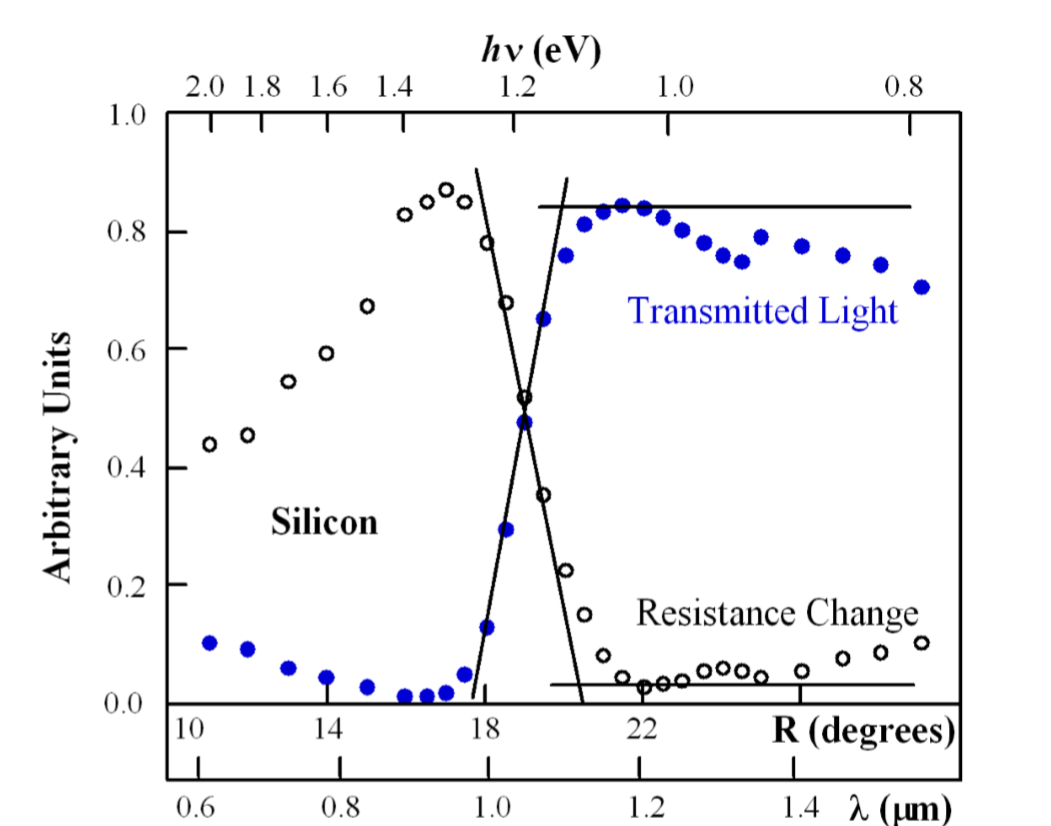
\includegraphics[scale=0.7]{Bilder/bsp_fit}
	\caption[Referenz zur Geraden Anpassung]{\small Beispiel zu den angepassten Geraden für die Bestimmung der Bandlückenenergie. Entnommen aus der Versuchsanleitung \cite{anleitung}}
	\label{anleitung_fit}	
\end{figure}

\subsection{Berechnung der Bandlückenenergie für Silizium}
Der erste Schritt bei der Normierung ist, die Messung der Lampe und die Silizium Messung auf die selbe Länge und Winkeländerung zu Synchronisieren. Die aufgezeichneten Messungen hatten leider beide obenerwähnten Änderungen, was korrigiert wurde. Es wurde begonnen, die ersten 18 zu verwerfen da hier keine Winkeländerung stattfindet. Als nun die Winkel zum Start der Daten nahezu übereinstimmten, wurde deutlich dass die Winkeländerungsrate der beiden Messungen unterschiedlich ist. Hierzu wurden bei einem Winkel in der Nähe von $0^{\circ}$ einige Datenpunkte ignoriert. Damit war die Anpassung abgeschlossen. Das Ergebnis der Anpassung ist in Abbildung \ref{anpassung_si_1} sichtbar. 

\begin{figure}[h]
	\centering

	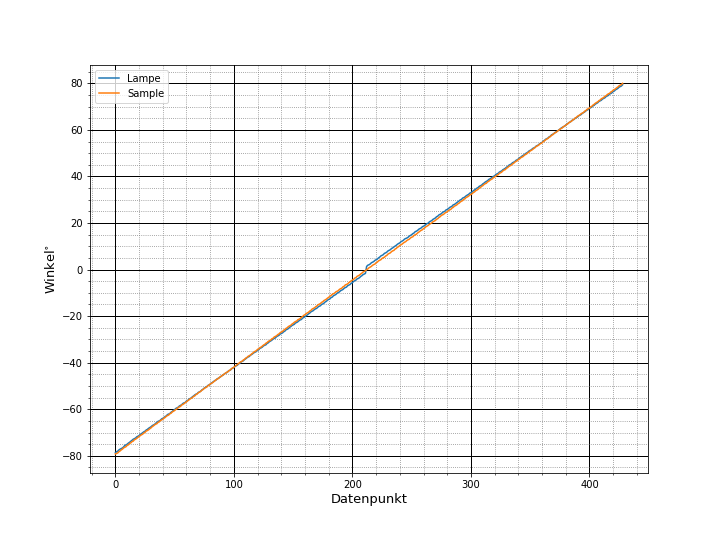
\includegraphics[scale=0.5]{Bilder/korrektur_channels}
	\caption[Korrigierter Lampendatensatz]{\small Auftragung der gemessenen Winkel für die Lampenmessung und erste Silizium Messung nach der Korrektur. Beide stimmen in den relevanten Bereichen bei ca. $30^{\circ}-40^{\circ}$ weitgehend überein.}	
	\label{anpassung_si_1}
\end{figure}

Es wurden mehrere Untergrundmessungen durchgeführt, wobei die ohne Gitter als am repräsentativsten gewählt wurde. Diese ist sichtbar in Abbildung \ref{untergrund} Da die Länge von der Untergrundmessung viel kürzer als die der eigentlichen Messungen, wurde bei dieser jeweils der Mittelwert als Repräsentation verwendet. 

\begin{figure}[h]
	\centering

	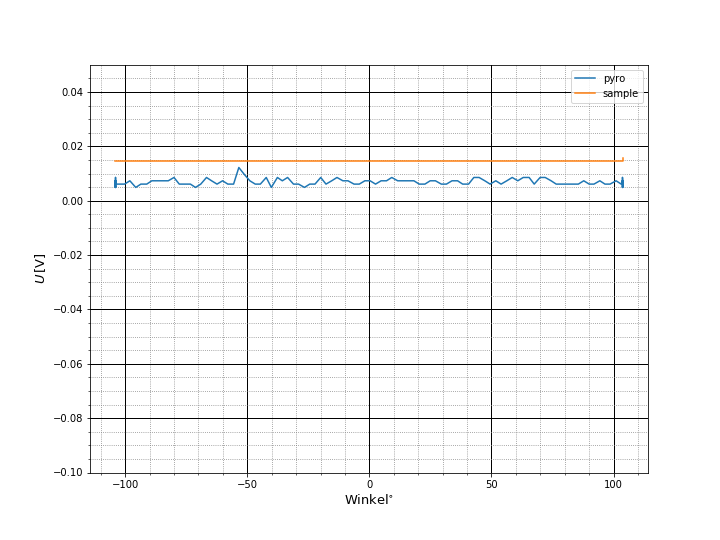
\includegraphics[scale=0.5]{Bilder/Hintergrund}
	\caption{\small Auftragung von gemessener Spannung der  Untergrundmessung gegen die Winkel.}
	\label{untergrund}	
\end{figure}

Das Ergebnis der Normalisierung ist in der Abbildung \ref{normalized} dargestellt.

\begin{figure}[h]
	\centering

	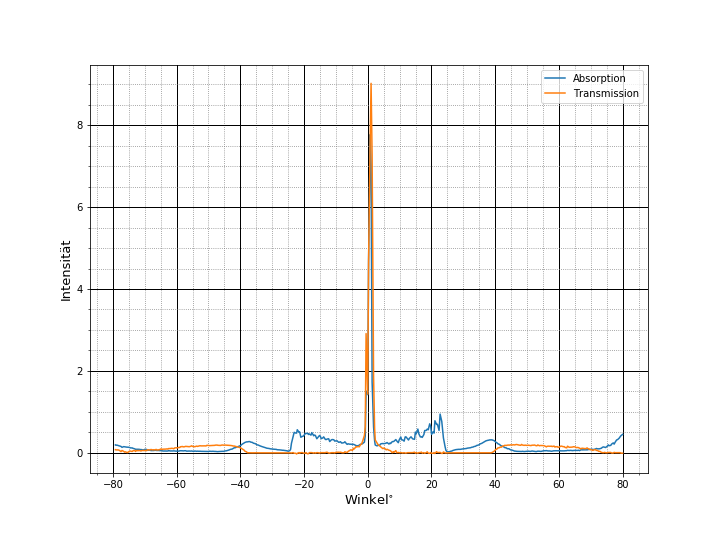
\includegraphics[scale=0.5]{Bilder/normalized}
	\caption{\small Auftragung von Intensität der normalisierten Datenreihen gegen die  Winkel.}
	\label{normalized}	
\end{figure}

Anschließend wurden die oben erwähnten Geraden angepasst. Dies wurde bei beiden Stellen der Messung durchgeführt. Anschließend wurden die Schnittpunkte der Geraden ($y = a\cdot +b$) mit den jeweiligen Horizontalen mittels der Formel \ref{schnitt} bestimmt. 
\begin{equation}
\label{schnitt}
x = \frac{x-b}{a}
\end{equation}
In Abbildungen \ref{si_1_l} und \ref{si_1_r} sind die angepassten Geraden, die horizontalen und deren Schnittpunkte dargestellt.
Die Parameter der Geraden, Horizontalen und die Winkel, bei welchen sie sich schneiden können aus der Tabelle \ref{ergebnis_si1} entnommen werden. Die so bestimmten Winkel der Schnittpunkte  wurden mit der Energie Datenreihe verglichen. Leider konnten sie nicht direkt abgelesen werden wegen der endlichen Genauigkeit der Aufgezeichneten Daten. Zunächst wurde versucht, eine Exponentialfunktion an die Daten anzupassen, was fehlschlug. Letztendlich wurde eine gerade an den Bereich angepasst, in welchem sich die Messwerte befinden. Diese sind in Abbildungen \ref{si_1_l_en} beispielhaft aufgetragen.

\begin{table}
	\centering
	\caption[Parameter erste Silizium Messung]{Parameter der angepassten Geraden, Horizontalen, Winkel der Schnittpunkte und die Energien zu den Schnittwinkeln der ersten Silizium Messung.}
	\label{ergebnis_si1}
	\begin{tabular}{lllll}
		\toprule
	Mess- &   Steigung und Offset  & Position der  & Winkel beim  & Energien der  \\
	reihe & der Geraden & Horizontalen & Schnittpunkt& Schnittpunkte in eV \\
	
	\midrule
		1. Absorbtion   &  [0.0273+/-0.0008, 1.261+/-0.033] &                 0.0281946 &                                -45.2+/-1.7 &               -1.06+/-0.04 \\
		1. Transmission &  [-0.0494+/-0.0026, -1.86+/-0.10] &                  0.190734 &                                -41.5+/-3.0 &               -1.13+/-0.06 \\
		2. Absorbtion   &   [-0.0370+/-0.0015, 1.73+/-0.06] &                 0.0309053 &                                 46.0+/-2.5 &                1.04+/-0.05 \\
		2. Transmission &   [0.0431+/-0.0026, -1.66+/-0.11] &                  0.204556 &                                     43+/-4 &                1.09+/-0.07 \\
		\bottomrule
	\end{tabular}
\end{table}

\begin{figure}[h]
	\centering

	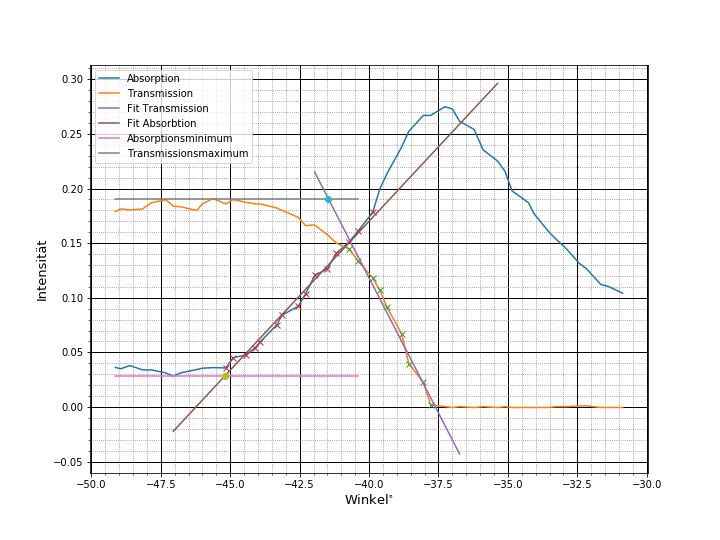
\includegraphics[scale=0.5]{Bilder/si_1_l}
	\caption[Geraden Anpassungen erste Silizium Messung links]{\small Auftragung von Intensität der normalisierten Datenreihen gegen die  Winkel der ersten Silizium Messung in der Nähe der Stelle Gleichwahrscheinlicher Absorption und Transmission bei Winkeln kleiner als $0^\circ$. Es sind zusätzlich die angepassten Geraden zur Absorption und Transmission eingezeichnet. Die Horizontalen wurden durch die Maxima der dahinterliegenden Datenpunkte bestimmt. Die Schnittpunkte der Geraden mit ihren jeweiligen Horizontalen sind auch eingezeichnet.}
	\label{si_1_l}
\end{figure}

\begin{figure}[h]
	\centering

	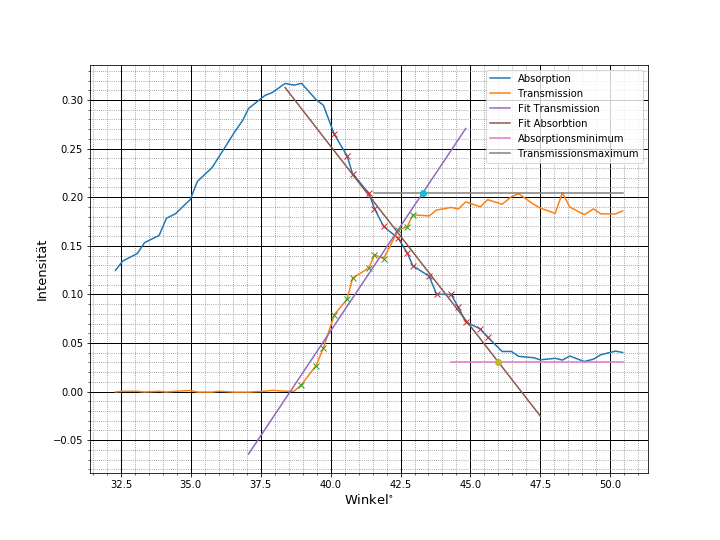
\includegraphics[scale=0.5]{Bilder/si_1_r}
	\caption[Geraden Anpassungen erste Silizium Messung rechts]{\small Auftragung von Intensität der normalisierten Datenreihen gegen die  Winkel der ersten Silizium Messung in der Nähe der Stelle Gleichwahrscheinlicher Absorption und Transmission bei Winkeln größer als $0^\circ$. Es sind zusätzlich die angepassten Geraden zur Absorption und Transmission eingezeichnet. Die Horizontalen wurden durch die Maxima der dahinterliegenden Datenpunkte bestimmt. Die Schnittpunkte der Geraden mit ihren jeweiligen Horizontalen sind auch eingezeichnet.}
	\label{si_1_r}	
\end{figure}

\begin{figure}[h]
	\centering

	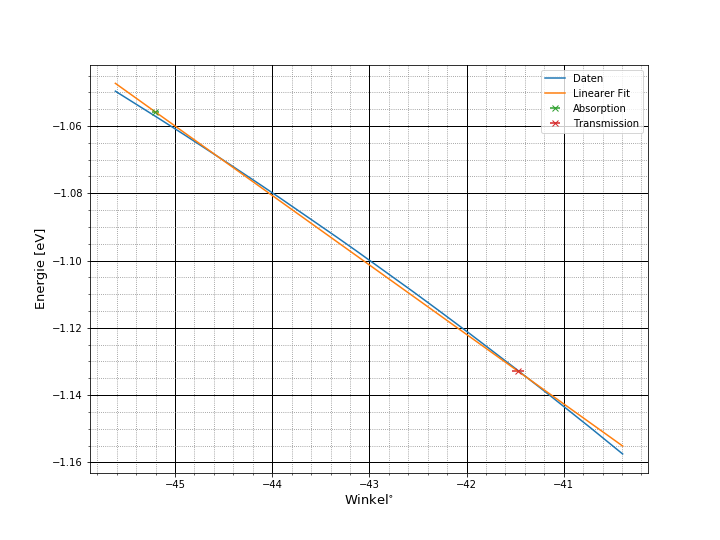
\includegraphics[scale=0.5]{Bilder/si_1_l_energie}
	\caption[Beispiel Energiebestimmung]{\small Auftragung der Energie gegen den Winkel. Die angepasste Gerade und die beiden Schnittpunkte sind auch eingetragen.}
	\label{si_1_l_en}	
\end{figure}

 Für die zweite Silizium Messung wurde nahezu analog vorgegangen. Es wurde zusätzlich eine Nullpunktkorrektur vorgenommen, da der Nullpunkt der Datenreihen deutlich von $0^\circ$ abwich. Die Korrektur betrug $-2.25^\circ$. Die Bilder zur Korrektur , den angepassten Geraden und der Energiebestimmung sind Anhang zu finden. Die Ergebnisse zur Auswertung stehen in Tabelle \ref{ergebnis_si2}.

 
 \begin{table}
 	\centering
 	\caption[Parameter der zweiten Silizium Messung]{Parameter der angepassten Geraden, Horizontalen, Winkel der Schnittpunkte und die Energien zu den Schnittwinkeln der zweiten Silizium Messung.}
 	\label{ergebnis_si2}
 	\begin{tabular}{lllll}
 		\toprule
 		Mess- &   Steigung und Offset  & Position der  & Winkel beim  & Energien der  \\
 		reihe & der Geraden & Horizontalen & Schnittpunkt& Schnittpunkte in eV \\
 		
 		\midrule
 		1. Absorbtion   &    [0.0327+/-0.0013, 1.49+/-0.05] &                 0.0274841 &                                -44.8+/-2.3 &               -1.11+/-0.05 \\
 		1. Transmission &  [-0.0398+/-0.0023, -1.49+/-0.09] &                  0.188553 &                                -42.2+/-3.3 &               -1.17+/-0.07 \\
 		2. Absorbtion   &   [-0.0418+/-0.0017, 1.94+/-0.07] &                 0.0300767 &                                 45.7+/-2.5 &                1.01+/-0.04 \\
 		2. Transmission &   [0.0486+/-0.0021, -1.88+/-0.09] &                  0.205715 &                                 42.9+/-2.6 &                1.06+/-0.04 \\
 		\bottomrule
 	\end{tabular}
 \end{table}

\subsection{Berechnung der Bandlückenenergie für Germanium}
Die Normierung von der Lampenmessung von Germanium war herausfordernder als die bisherigen, da hier die Lampenmessung nicht nur eine unterschiedliche Länge hatte sondern auch eine größere Winkeländerungsdifferenz. Nachdem die Reihenfolge der Daten umgekehrt wurde, wurden immer wieder kleine Teile des Datensatzes ignoriert, dass sich der Datensatz von Lampe und der eigentlichen Messung besser angleichen. Das ist in Abbildung \ref{ge_korr_lamp} dargestellt. 


\begin{figure}[h]
	\centering
	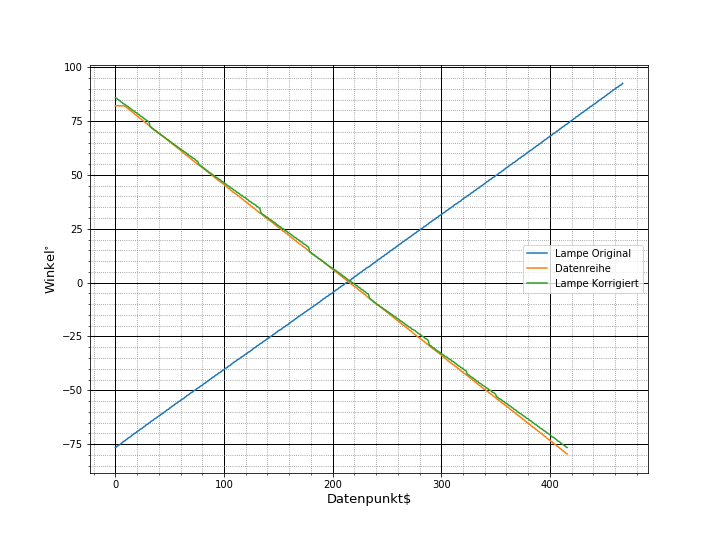
\includegraphics[scale=0.5]{Bilder/Korrektur_ge}
	\caption[Korrektur der Lampendaten Germanium]{\small Hier sind die Winkel der Original Lampendaten, die Daten der Messung und die Korrigierten Lampendaten gegen die Stellen der Datenpunkte aufgetragen.}
	\label{ge_korr_lamp}	
\end{figure}

Die restlichen Teile der Auswertung verliefen analog zu den Silizium Auswertungen. Die angepassten Geraden sind in Abbildung \ref{fit_ger} zu sehen, die Ergebnisse in Tabelle \ref{ergebnis_ge}.

\begin{figure}[h]


	\centering
	
	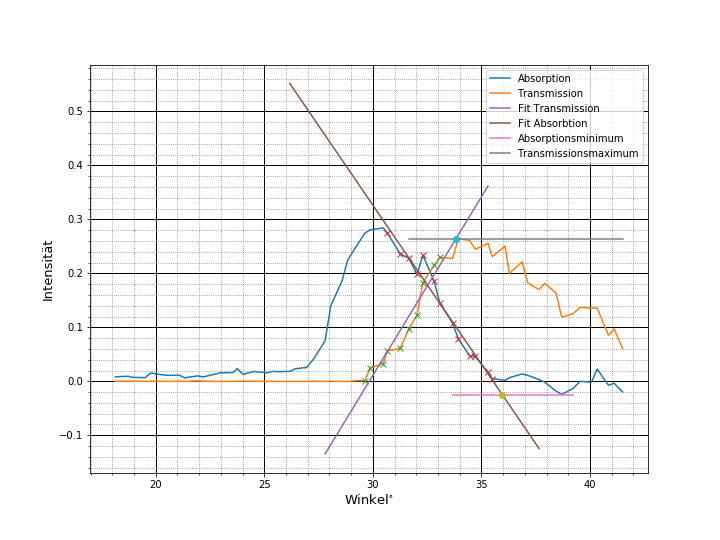
\includegraphics[scale=0.5]{Bilder/ge_l}
	\caption[Geraden Anpassungen Germanium Messung links]{\small Auftragung von Intensität der normalisierten Datenreihen von Germanium gegen die  Winkel in der Nähe der Stelle Gleichwahrscheinlicher Absorption und Transmission bei Winkeln größer als $0^\circ$. Es sind zusätzlich die angepassten Geraden zur Absorption und Transmission eingezeichnet. Die Horizontalen wurden durch die Maxima der dahinterliegenden Datenpunkte bestimmt. Die Schnittpunkte der Geraden mit ihren jeweiligen Horizontalen sind auch eingezeichnet.}
	\label{fit_ger}	
\end{figure}

 \begin{table}
	\centering
	\caption[Parameter der zweiten Silizium Messung]{Parameter der angepassten Geraden, Horizontalen, Winkel der Schnittpunkte und die Energien zu den Schnittwinkeln der zweiten Silizium Messung.}
	\label{ergebnis_ge}
	\begin{tabular}{lllll}
		\toprule
		Mess- &   Steigung und Offset  & Position der  & Winkel beim  & Energien der  \\
		reihe & der Geraden & Horizontalen & Schnittpunkt& Schnittpunkte in eV \\
		
		\midrule
		1. Absorbtion   &   [-0.0589+/-0.0033, 2.09+/-0.11] &                -0.0245099 &                                 36.0+/-2.7 &                0.64+/-0.05 \\
		1. Transmission &     [0.066+/-0.006, -1.97+/-0.19] &                  0.263931 &                                     34+/-4 &                0.68+/-0.07 \\
		2. Absorbtion   &      [0.073+/-0.005, 2.58+/-0.15] &                -0.0239853 &                                -35.7+/-3.1 &               -0.64+/-0.05 \\
		2. Transmission &  [-0.0817+/-0.0030, -2.46+/-0.10] &                  0.552449 &                                -36.9+/-1.9 &             -0.625+/-0.029 \\
		\bottomrule
	\end{tabular}
\end{table}	